%%%%%%%%%%%%%%%%%%%%[Free to change]%%%%%%%%%%%%%%%%%%%%
% Starting from February 2021, SNU students are no longer required to submit a printed dissertation; only a digital version is necessary. Consequently, the library no longer enforces strict rules for page size, margin size, fonts, and font sizes. Their guidance is to "basically follow the template." Therefore, all parameters (including code lines) within this %%%%[Free to change]%%%% block can be adjusted by the student as desired, as long as it doesn't significantly compromise readability.

% """중앙도서관에서 LaTex 양식은 별도로 제공하고 있지 않으며, word / 한글 양식만 제공하고 있는 점 양해 부탁드립니다. [...] 현재 저희가 제공하고 있는 작성 요령 및 내용 구성 등은 기본적으로 따르되, 많이 문의해주시는 논문의 규격(본문 크기, 여백 등), 서체(활자 종류 및 크기)에 대해서는 엄격하게 규정해두고 있지 않은 점 알려드립니다."""  - email by libit@snu.ac.kr on 2022-12-05 to ysBach.
%%%%%%%%%%%%%%%%%%%%%%%%%%%%%%%%%%%%%%%%%%%%%%%%%%%%%%%%

\documentclass[12pt]{report}
\usepackage[paperwidth=21cm,paperheight=29.7cm,left=2.5cm,right=2.5cm,top=3.5cm,bottom=1.5cm]{geometry}
% Originally this was
%\usepackage[paperwidth=19cm,paperheight=26cm,left=3cm,right=3cm,top=3.5cm,bottom=1.5cm]{geometry}

\addtolength{\voffset}{-1.5cm}
\renewcommand{\baselinestretch}{1.7}
\renewcommand{\abstractname}{\large Abstract}
\usepackage{setspace}
\usepackage[]{enumitem}
%\usepackage{lmodern}
%\usepackage{librecaslon}
\usepackage[T1]{fontenc}
\usepackage{footnote}
\usepackage{textcomp}
\usepackage{kotex}

% ↓ This is also free to change. Do as you wish...
\usepackage[
  round,
  semicolon,
  authoryear,
%  sort
]{natbib}


%%%%%%%%%%%%%%%%%%%%
% For proper page numbering at TOC part https://tex.stackexchange.com/questions/235866/page-number-resets-on-table-of-contents
\makeatletter
\renewenvironment{abstract}{%
    \if@twocolumn
    \section*{\abstractname}%
    \else
    \small
    \begin{center}%
        {\bfseries \abstractname\vspace{-.5em}\vspace{\z@}}%
    \end{center}%
    \quotation
    \fi}
{\if@twocolumn\else\endquotation\fi}
\makeatother
%%%%%%%%%%%%%%%%%%%%

%↓↓↓↓↓↓↓↓↓↓[Free to change, preamble. START]↓↓↓↓↓↓↓↓↓↓
% It is your choice to change contents from here to the end of preamble.

\usepackage{amsmath,amssymb}
\usepackage{tikz}
\usepackage{mathtools}
\usepackage{graphicx}
\usepackage{siunitx}
\usepackage{physics}
\usepackage{rotating}  % The package to rotate table by sidewaystable
\usepackage{csquotes}  % for ``displayquote`` environment
\usepackage[notextcomp]{stix}  % without notextcomp, "Option clash for package textcomp." error pops up...
%\usepackage[libertine,cmintegrals,cmbraces,vvarbb]{newtxmath}
\usepackage[font=small]{caption}
\usepackage{listings}
\usepackage{xcolor}


%%%%%%%%%%%%%%%%%%%%
% For URL-ed A&A style bibliography (https://github.com/yangcht/AA-bibstyle-with-hyperlink)
% IMPORTANT NOTE:
% As of 2023-05-18, at least PHDTHESIS must have `adsurl={}` and `adsnote={}`, when they are not registered to ADS. If they don't have these fields, """Extra }, or forgotten \endgroup. """ error will appear.
\usepackage{twoopt}
\usepackage[breaklinks]{hyperref}      %% to avoid \citeads line fills, add "draft"
                                       %% to avoid the PDFTK error (broken links)
\bibpunct{(}{)}{;}{a}{}{,}             %% natbib format for A&A and ApJ
\definecolor{cobalt}{rgb}{0.06, 0.2, 0.65}
\hypersetup{
  colorlinks,
  citecolor=cobalt,
  linkcolor=[rgb]{0.8, 0.2, 1.0},
  urlcolor=cobalt,
}
\makeatletter
  \newcommandtwoopt{\citeads}[3][][]{\href{http://adsabs.harvard.edu/abs/#3}%
    {\def\hyper@linkstart##1##2{}%
     \let\hyper@linkend\@empty\citealp[#1][#2]{#3}}}
  \newcommandtwoopt{\citepads}[3][][]{\href{http://adsabs.harvard.edu/abs/#3}%
    {\def\hyper@linkstart##1##2{}%
     \let\hyper@linkend\@empty\citep[#1][#2]{#3}}}
  \newcommandtwoopt{\citetads}[3][][]{\href{http://adsabs.harvard.edu/abs/#3}%
    {\def\hyper@linkstart##1##2{}%
     \let\hyper@linkend\@empty\citet[#1][#2]{#3}}}
  \newcommandtwoopt{\citeyearads}[3][][]%
    {\href{http://adsabs.harvard.edu/abs/#3}
    {\def\hyper@linkstart##1##2{}%
     \let\hyper@linkend\@empty\citeyear[#1][#2]{#3}}}
\makeatother
%%%%%%%%%%%%%%%%%%%%

\usepackage{url}
%\usepackage{hyperref}
\usepackage{cleveref}

%\crefname{equation}{equation}{equations}%
%\crefname{chapter}{chapter}{chapters}%
%\crefname{section}{section}{sections}%
%\crefname{appendix}{appendix}{appendices}%
%\crefname{enumi}{item}{items}%
%\crefname{footnote}{footnote}{footnotes}%
%\crefname{figure}{figure}{figures}%
%\crefname{table}{table}{tables}%
%\crefname{theorem}{theorem}{theorems}%
%\crefname{lemma}{lemma}{lemmas}%
%\crefname{corollary}{corollary}{corollaries}%
%\crefname{proposition}{proposition}{propositions}%
%\crefname{definition}{definition}{definitions}%
%\crefname{result}{result}{results}%
%\crefname{example}{example}{examples}%
%\crefname{remark}{remark}{remarks}%
%\crefname{note}{note}{notes}%

\Crefname{equation}{Eq.}{Eqs.}%
\Crefname{chapter}{Chap.}{Chaps.}%
\Crefname{section}{\S}{\S}%
\Crefname{appendix}{App.}{Apps.}%
\Crefname{enumi}{item}{items}%
\Crefname{footnote}{footnote}{footnotes}%
\Crefname{figure}{Fig.}{Figs.}%
\Crefname{table}{Tab.}{Tabs.}%
%\Crefname{theorem}{Thm.}{Thms.}%
%\Crefname{lemma}{Lem.}{Lems.}%
%\Crefname{corollary}{Cor.}{Cors.}%
%\Crefname{proposition}{proposition}{propositions}%
\Crefname{definition}{Def.}{Defs}%
%\Crefname{result}{result}{results}%
%\Crefname{example}{example}{examples}%
%\Crefname{remark}{remark}{remarks}%
%\lCrefname{note}{note}{notes}%

\makeatletter
\renewcommand*{\fps@figure}{tb}
\renewcommand*{\fps@table}{tb}
\makeatother

\renewenvironment{abstract}
 {\small
  \begin{center}
  \bfseries \abstractname\vspace{-.5em}\vspace{0pt}
  \end{center}
  \list{}{%
    \setlength{\leftmargin}{10mm}% <---------- CHANGE HERE
    \setlength{\rightmargin}{\leftmargin}%
  }%
  \item\relax}
 {\endlist}

%↑↑↑↑↑↑↑↑↑↑[Free to change, preamble. END]↑↑↑↑↑↑↑↑↑↑

\begin{document}

\pagenumbering{gobble}

\begin{titlepage}
\def\tTitleA{{On the Physical Behavior of}}
\def\tTitleB{{Fine Particles on Airless Bodies}}
\def\tTitleK{{대기 없는 천체 위에서 고운 입자의 \\물리적 행동에 관하여}}
\def\tDepartment{{물리$\cdot$천문학부}}
\def\tDate{{2023년 5월}}
\def\tName{{Yoonsoo P. Bach}}
\def\tNameWithBlank{{Yoonsoo P. Bach}}

\renewcommand{\baselinestretch}{1}
\centering
{\Large \quad \par}
\vspace{.5cm}
{\Large 이학박사 학위논문 \par}
\vspace{2cm}
{\Huge \tTitleA \par}
\vspace{.3cm}
{\Huge \tTitleB \par}
\vspace{2cm}
{\LARGE \tTitleK \par}
\vspace{4.5cm}
{\Large \tDate \par}
\vspace{3cm}
{\LARGE 서울대학교 대학원 \par}
\vspace{.5cm}
{\Large \tDepartment \par}
\vspace{.5cm}
{\LARGE \tNameWithBlank \par}

\clearpage

\centering
{\Large \quad \par}
\vspace{.1cm}
{\Huge \tTitleA \par}
\vspace{.3cm}
{\Huge \tTitleB \par}
\vspace{1.5cm}
{\LARGE 지도교수 $\ $ Masateru $\ $ Ishiguro \par}
\vspace{1cm}
{\LARGE 이 논문을 이학박사 학위논문으로 제출함 \par}
\vspace{.2cm}
{\Large \tDate \par}

\vspace{.9cm}
{\LARGE 서울대학교 대학원 \par}
\vspace{.3cm}
{\Large \tDepartment \par}
\vspace{.3cm}
{\LARGE \tNameWithBlank \par}
\vspace{.9cm}

{\LARGE \tName의 박사 학위논문을 인준함 \par}
\vspace{.2cm}
{\Large \tDate \par}
\vspace{1.2cm}
{\Large 위\hspace{.255cm}원\hspace{.255cm}장} \quad {\Large \underline{\qquad\qquad\qquad\qquad\qquad(인)} } \par
\vspace{.3cm}
{\Large 부위원장} \quad {\Large \underline{\qquad\qquad\qquad\qquad\qquad(인)} } \par
\vspace{.3cm}
{\Large 위\hspace{1cm}원} \quad {\Large \underline{\qquad\qquad\qquad\qquad\qquad(인)} } \par
\vspace{.3cm}
{\Large 위\hspace{1cm}원} \quad {\Large \underline{\qquad\qquad\qquad\qquad\qquad(인)} } \par
\vspace{.3cm}
{\Large 위\hspace{1cm}원} \quad {\Large \underline{\qquad\qquad\qquad\qquad\qquad(인)} } \par 
\end{titlepage}

%↓↓↓↓↓↓↓↓↓↓[Free to change, settings/macro START]↓↓↓↓↓↓↓↓↓↓

\setstretch{1.3}  % 1.3 is good because (1) it is not too large, but (2) large enough that a simple inline fraction ($\frac{num}{den}$) is well displayed.
\renewcommand*{\bibfont}{\normalfont\small}
\setlength{\bibsep}{10pt plus 1em}
\setlength{\parindent}{2em}
\setlength{\parskip}{0.5em}

%%%%%%%%%%%%%%%%%%%%[    MACROS    ]%%%%%%%%%%%%%%%%%%%%
\renewcommand{\thefootnote}{\alph{footnote}}
\renewcommand{\lg}{\ensuremath{\log_{10}}}
\newcommand{\thru}{\ensuremath{\text{--}}}

\renewcommand{\pV}{\ensuremath{p_\mathrm{V}}}
\newcommand{\HV}{\ensuremath{H_\mathrm{V}}}
\newcommand{\HVa}{\ensuremath{H_\mathrm{V}(\alpha)}}
\newcommand{\Prot}{\ensuremath{P_\mathrm{rot}}}
%\newcommand{\earth}{\ensuremath{_\oplus}}
%\newcommand{\sun}{\ensuremath{_\odot}}

\newcommand{\solarconst}{\ensuremath{\SI{1361.2}{W/m^2}}}
\newcommand{\SB}{\ensuremath{\sigma_\mathrm{SB}}}
\newcommand{\kB}{\ensuremath{k_\mathrm{B}}}
\newcommand{\rhel}{\ensuremath{r_\mathrm{hel}}}
\newcommand{\robs}{\ensuremath{r_\mathrm{obs}}}
\newcommand{\sr}{\ensuremath{\,\mathrm{sr}}}
\newcommand{\fwhm}{\ensuremath{\textsc{FWHM}}}
\newcommand{\hwhm}{\ensuremath{\textsc{HWHM}}}

\newcommand{\degr}{\ensuremath{^\circ}}
\renewcommand{\um}{\ensuremath{\,\mathrm{\mu m}}}
\renewcommand{\nm}{\ensuremath{\,\mathrm{nm}}}
\renewcommand{\Angstrom}{\ensuremath{\,\text{\r{A}}}}
\renewcommand{\mm}{\ensuremath{\,\mathrm{mm}}}
\renewcommand{\cm}{\ensuremath{\,\mathrm{cm}}}
\renewcommand{\km}{\ensuremath{\,\mathrm{km}}}
\newcommand{\au}{\ensuremath{\,\mathrm{au}}}
\newcommand{\mden}{\ensuremath{\,\mathrm{kg\,m^{-3}}}}
\newcommand{\hr}{\ensuremath{\,\mathrm{hr}}}
\newcommand{\yr}{\ensuremath{\,\mathrm{yr}}}

\newcommand{\sep}{\quad;\quad}
\newcommand{\separr}{\quad \rightarrow \quad}
\newcommand{\simdot}{\mathrel{\dot{\sim}}}

\newcommand{\lineseg}[1]{\ensuremath{\overline{\mathrm{#1}}}}
\newcommand{\triang}[1]{\ensuremath{\triangle \mathrm{#1}}}
\newcommand{\rect}[1]{\ensuremath{\Box \mathrm{#1}}}
\newcommand{\linevec}[1]{\ensuremath{\overrightarrow{\mathrm{#1}}}}


\newcommand{\chapquote}[2]{\qquad\textit{#1} \begin{flushright} --- #2\end{flushright} }

%https://tex.stackexchange.com/questions/19605/setting-arbitrary-chapter-values
\newcommand{\strangechapter}[1]{\renewcommand{\thechapter}{#1}\chapter*}

\newcommand{\kr}[1]{{\scriptsize #1}}  % Just... to reduce font size for Hangeul characters in Acknowledgement.
%%%%%%%%%%%%%%%%%%%%%%%%%%%%%%%%%%%%%%%%%%%%%%%%%%%%%%%%
%%% for python
\definecolor{codegreen}{rgb}{0,0.6,0}
\definecolor{codegray}{rgb}{0.5,0.5,0.5}
\definecolor{codepurple}{rgb}{0.58,0,0.82}
\definecolor{backcolour}{rgb}{0.95,0.95,0.92}
\lstdefinelanguage{none}{
  identifierstyle=
}
\lstdefinestyle{python}{  % https://en.wikibooks.org/wiki/LaTeX/Source_Code_Listings
    backgroundcolor=\color{backcolour}, % choose the background color; you must add \usepackage{color} or \usepackage{xcolor}; should come as last argument
    commentstyle=\color{codegreen},     % comment style
    keywordstyle=\color{magenta},
    numberstyle=\tiny\color{codegray},
    stringstyle=\color{codepurple},
    basicstyle=\ttfamily\scriptsize, % the size of the fonts that are used for the code
    breakatwhitespace=false,           % sets if automatic breaks should only happen at whitespace
    breaklines=true,                   % sets automatic line breaking
%    captionpos=b,                      % sets the caption-position to bottom
    keepspaces=true,                   % keeps spaces in text, useful for keeping indentation of code (possibly needs columns=flexible)
%    numbers=left,                    % where to put the line-numbers; possible values are (none, left, right)
%    numbersep=5pt,                   % how far the line-numbers are from the code
%    numberstyle=\tiny\color{mygray}, % the style that is used for the line-numbers
%    stepnumber=10,                    % the step between two line-numbers. If it's 1, each line will be numbered
    showspaces=false,                % show spaces everywhere adding particular underscores; it overrides 'showstringspaces'
    showstringspaces=false,          % underline spaces within strings only
    showtabs=false,
    rulecolor=\color{black},         % if not set, the frame-color may be changed on line-breaks within not-black text (e.g. comments (green here))
    tabsize=2,                        % sets default tabsize to 2 spaces
    showtabs=false,                  % show tabs within strings adding particular underscores
    language=Python,                 % the language of the code
%    stringstyle=\color{mymauve},     % string literal style
%    title=\lstname,                   % show the filename of files included with \lstinputlisting; also try caption instead of title
%    deletekeywords={...},            % if you want to delete keywords from the given language
%    escapeinside={\%*}{*)},          % if you want to add LaTeX within your code
%    extendedchars=true,              % lets you use non-ASCII characters; for 8-bits encodings only, does not work with UTF-8
%    firstnumber=1000,                % start line enumeration with line 1000
%    frame=single,	                   % adds a frame around the code
%    keywordstyle=\color{blue},       % keyword style
%    morekeywords={*,...},            % if you want to add more keywords to the set
    upquote=true
}

\lstset{style=python}
%↑↑↑↑↑↑↑↑↑↑[Free to change, settings/macros. END]↑↑↑↑↑↑↑↑↑↑




\begin{abstract}
\addcontentsline{toc}{chapter}{Abstract}
\pagenumbering{roman}
%\setcounter{page}{4}
Starting from February 2021, SNU students are no longer required to submit a printed dissertation; only a digital version is necessary (printed version is actually not allowed). Consequently, the library no longer enforces strict rules for page size, margin size, fonts, and font sizes. They replied ``{\footnotesize 중앙도서관에서 LaTeX 양식은 별도로 제공하고 있지 않으며, word / 한글 양식만 제공하고 있는 점 양해 부탁드립니다. [...] 현재 저희가 제공하고 있는 작성 요령 및 내용 구성 등은 기본적으로 따르되, 많이 문의해주시는 논문의 규격(본문 크기, 여백 등), 서체(활자 종류 및 크기)에 대해서는 엄격하게 규정해두고 있지 않은 점 알려드립니다.}'' - email by libit@snu.ac.kr on 2022-12-05 to ysBach.

\quad Their guidance is to ``follow the template'' but you can modify as you wish. Therefore, all parameters (including code lines) within this TeX source code, especially indicated by \texttt{\%\%\%\%[Free to change]\%\%\%\%} block, can be adjusted by the student as desired, as long as it doesn't significantly compromise readability. Please look into the main manuscript TeX file. Prior to Feb 2021, regulations were based on the commercial HWP processor. Among them, regulation for main text: \textcolor{red}{(I repeat again: \textbf{regulations stated below can be adjusted by the student as desired}, as long as it doesn't significantly compromise readability)}
\begin{enumerate}[itemsep=0pt, topsep=0pt, partopsep=0pt]
\item Print the text in 38 characters x 25 lines.
\item The amount of text is free based on the size of the paper (19 cm × 26 cm).
\item Text: font size around 11pt, line spacing 170 or more (in HWP), justification (horizontal separation of characters in HWP) 100, ruled (vertical separation of characters in HWP) 0
\item Footnotes: font size 9~10pt
\item Typeface: Myeongjo (명조체) or neo-myeongjo (shin-myeongjo 신명조체) type
\item Font color: Black (color is available for included materials)
\item Paper margins: top 20, bottom 15, header 15, footer 15, left 30, right 30 (in HWP)
\item Page marks should be centered at the bottom of each side.
\end{enumerate}
and regulation for the Abstract (which seems to include title pages too):
\begin{enumerate}[itemsep=0pt, topsep=0pt, partopsep=0pt]
\item The abstract should be written in one of the following languages: English, Japanese, French, or German if the main text is in Korean.
\item If the paper is written in non-Korean, it must be accompanied by a Korean abstract.
\item The length of the abstract should be within 2-7 pages.
\item The title of the abstract should be in the original language. If this is not possible to make it one-line, the second line should be centered.
\item The subtitle should be centered at the bottom of the title.
\item Include your full name, major, department, and school name at the bottom of the title.
\item At the bottom of the abstract, include within(?) 7-8 keywords that indicate the topic of your paper.
\end{enumerate}
For abstract and keywords, there's another set of notes as of 2023 Aug:
\begin{enumerate}[itemsep=0pt, topsep=0pt, partopsep=0pt]
\item Keywords are words or phrases that indicate the core content of the paper.
\item Select within(?) 7-8 keywords that can be used as index words when searching for a paper. Present them at the end of the abstract.
\item Keywords should be written in the same language as the abstract.
\item The most relevant keyword to the topic of the paper should come first.
\item In English, the first paragraph is usually not indented, and later paragraphs are indented.
\end{enumerate}
For specific formatting details, please consult the official announcement from the library. However, note that you do not need to adhere to their guidelines ``exactly,'' especially since they do not even provide a LaTeX template. I have seen hundreds of theses which goes completely against the official format. The ``tradition'' among your department upper classmates is the most reliable format.

\quad Normally, the order of contents should follow:
\begin{enumerate}[itemsep=0pt, topsep=0pt, partopsep=0pt]
\item Outer cover (Not necessary after Feb 2021)
\item Blank page (Not necessary after Feb 2021)
\item Title page
\item Approval page (called ``인준지'')
\item Abstract (in the language of the main text)
\item Table of contents (including list of tables, list of figures, etc.)
\item Main text
\item References
\item Appendices, index, other (if necessary)
\item Second language abstract (Korean abstract if the text is in a non-Korean language)
\item Acknowledgments (may be omitted)
\item Blank page (Not necessary after Feb 2021)
\item Back cover (Not necessary after Feb 2021)
\end{enumerate}

Please be aware that regulations may change in the future. It is your responsibility to verify the regulations in effect at the time of your submission.


\hangindent=2em
\hangafter=2
\textbf{Keywords}: Asteroids, Regolith, Thermal modeling, Radiation Pressure, Polarimetry---Optical, Polarimetry---Infrared

~\\
\noindent \textbf{\textit{Student Number}}: 2016-20329

\end{abstract}


%%%%%%%%%%%%%%%%%%%%%%%%%%%%%%%%%%%%%%%%%%%%%%%%%%%%%%%%%
%% For page numbering of Abstract & TOC
%\newcounter{mypageno}
%\let\oldtableofcontents\tableofcontents
%\renewcommand{\tableofcontents}{%
%  \oldtableofcontents
%  \cleardoublepage
%  \setcounter{mypageno}{\value{page}}%
%  \pagenumbering{roman}%
%  \setcounter{page}{\value{mypageno}}%
%}
%%%%%%%%%%%%%%%%%%%%%%%%%%%%%%%%%%%%%%%%%%%%%%%%%%%%%%%%%
{
\setstretch{1.}
\setcounter{tocdepth}{2}
\tableofcontents
\addtocontents{lof}{\protect\addcontentsline{toc}{chapter}{List of Figures}}
\listoffigures
\addtocontents{lot}{\protect\addcontentsline{toc}{chapter}{List of Tables}}
\listoftables
}

\chapter*{List of Acronyms}\addcontentsline{toc}{chapter}{List of Acronyms}
\noindent\textbf{AR}: Asteroid Regolith
\\
\noindent\textbf{IAU}: International Astronomical Union
\\
\noindent\textbf{NEOs}: Near-Earth Objects
\\
\noindent\textbf{NEAs}: Near-Earth Asteroids
\\
\noindent\textbf{NEATM}: Near-Earth Asteroid Thermal Model
\\
\noindent\textbf{NIR}: Near-InfraRed
\\
\noindent\textbf{PCA}: Principal Component Analyses
\\
\noindent\textbf{PPC}: Polarimetric Phase Curve, $P_\mathrm{r}(\alpha)$
\\
\noindent\textbf{SSSB}: Small Solar System Bodies
\\
\noindent\textbf{STM}: Standard Thermal Model
\\
\noindent\textbf{TPM}: ThermoPhysical Model
\\
\noindent\textbf{YORP}: Yarkovsky--O'Keefe--Radzievskii--Paddack (effect)

\clearpage

~ \\ ~ \\ ~ \\
\begin{center}
\textbf{\textit{
To humanity and the giants
%who never faltered in their contemplation of the world, \\
%enduring the trials to uphold their conscientious attitude \\
%towards building scientific knowledge.
}}
\end{center}

\mbox{}
\vfill
{\noindent Science knows no country, \\ because knowledge belongs to humanity, \\ and is the torch which illuminates the world.}

{\footnotesize
%\noindent Science is the highest personification of the nation
%\\ \noindent because that nation will remain the first
%\\ \noindent which carries the furthest the works of thought and intelligence.
}

\hfill ---\textit{Louis Pasteur}
\clearpage


\pagenumbering{arabic}
\part{Backgrounds}\label{part-bkg}

\chapter{Introduction}\label{c:intro}
\chapquote{Natura non facit saltus.}{Gottfried Leibniz}
This is the introduction. For \texttt{itemize} or \texttt{enumerate}, you may tune the separations:
\begin{itemize}
\item This is the original itemize. Enumerate should look similar, but with numbers for \texttt{$\backslash$item}.
\item This is a long item to show how it will look like. This is a long item to show how it will look like. This is a long item to show how it will look like.
\item Short item.
\item Short item.
\item Short item.
\end{itemize}

You may add something like \texttt{[itemsep=-5pt, topsep=0pt, partopsep=0pt]} to make it tighter:
\begin{itemize}[itemsep=-5pt, topsep=0pt, partopsep=0pt]
\item This is the original itemize. Enumerate should look similar, but with numbers for \texttt{$\backslash$item}.
\item This is a long item to show how it will look like. This is a long item to show how it will look like. This is a long item to show how it will look like.
\item Short item.
\item Short item.
\item Short item.
\end{itemize}

In this thesis, the preamble includes
\begin{itemize}[itemsep=-5pt, topsep=0pt, partopsep=0pt]
\item Font STIX: ``\texttt{usepackage[notextcomp]\{stix\}}''
\item natbib: ``\texttt{usepackage[round,semicolon,authoryear]\{natbib]\}}''
\item Small caption: ``\texttt{usepackage[font=small]\{caption\}}''
\item Some useful packages: siunitx, physics, rotating (The package to rotate table by sidewaystable), csquotes (for ``displayquote'' environment), listings
\item Then a preamble for URLed A\&A bibliography (see \Cref{ss:ref style}).
\item Then a preamble for cleveref (see \Cref{ss:cref}).
\item Then a preamble for List of Figures \& List of Tables.
\item Then a preamble for the first language abstract.
\item Then a preamble for the page numbering, page margin, \texttt{setlength}, etc, as well as MACROs.
\end{itemize}



\chapter{Figure and Table}
\chapquote{God does not care about our mathematical difficulties.}{Albert Einstein}
This chapter briefly describes how to insert figures and tables (especially those that are rotated 90 degrees, which are very common in theses).

\section{Figure}
When you want to create a TikZ figure, you can use the online tool \texttt{Mathcha.io}\footnote{\url{https://www.mathcha.io/editor}}.


\begin{figure}
\centering
\tikzset{every picture/.style={line width=0.75pt}} %set default line width to 0.75pt
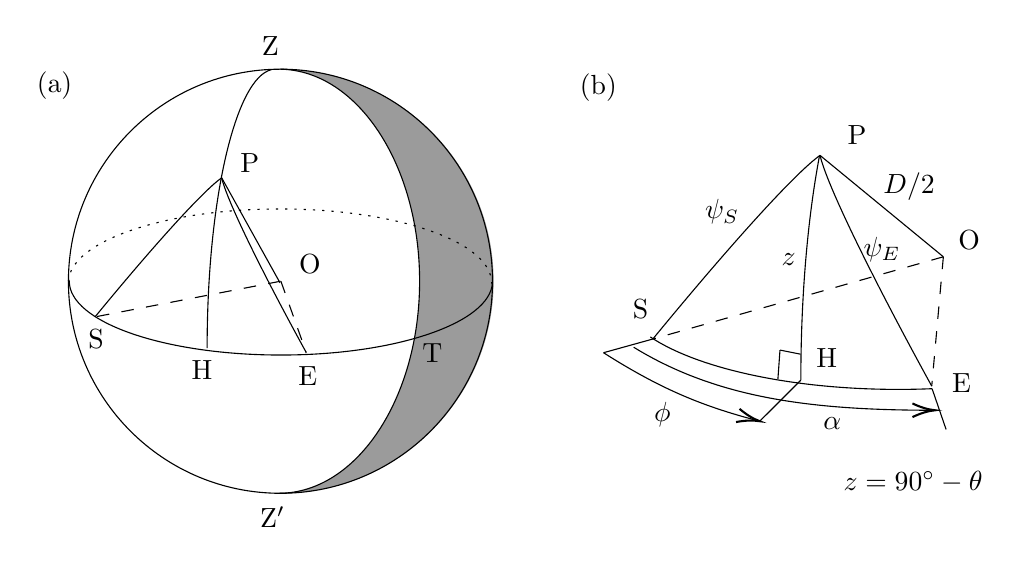
\begin{tikzpicture}[x=0.75pt,y=0.75pt,yscale=-1,xscale=1]

%uncomment if require:\path (0,476.33333587646484); %set diagram left start at 0, and has height of 476.33333587646484

%Shape:Arc [id:dp9200567780243829]
\draw  [draw opacity=0][fill={rgb, 255:red, 155; green, 155; blue, 155 }  ,fill opacity=1 ] (189.77,24) .. controls (246.05,24.43) and (291.54,70) .. (291.54,126.16) .. controls (291.54,182.44) and (245.87,228.08) .. (189.43,228.33) -- (188.96,126.16) -- cycle ; \draw  [draw opacity=0] (189.77,24) .. controls (246.05,24.43) and (291.54,70) .. (291.54,126.16) .. controls (291.54,182.44) and (245.87,228.08) .. (189.43,228.33) ;
%Shape:Arc [id:dp7489325740381287]
\draw  [draw opacity=0][fill={rgb, 255:red, 255; green, 255; blue, 255 }  ,fill opacity=1 ] (188.83,24) .. controls (225.93,24.65) and (255.87,70.14) .. (255.87,126.16) .. controls (255.87,182.36) and (225.75,227.96) .. (188.49,228.33) -- (188.03,126.16) -- cycle ; \draw   (188.83,24) .. controls (225.93,24.65) and (255.87,70.14) .. (255.87,126.16) .. controls (255.87,182.36) and (225.75,227.96) .. (188.49,228.33) ;
%Shape:Circle [id:dp03629587840911208]
\draw   (86.67,126.17) .. controls (86.67,69.74) and (132.41,24) .. (188.83,24) .. controls (245.26,24) and (291,69.74) .. (291,126.17) .. controls (291,182.59) and (245.26,228.33) .. (188.83,228.33) .. controls (132.41,228.33) and (86.67,182.59) .. (86.67,126.17) -- cycle ;
%Shape:Arc [id:dp7942338684517938]
\draw  [draw opacity=0] (290.97,126.89) .. controls (289.85,146.19) and (244.64,161.72) .. (189.04,161.72) .. controls (132.73,161.72) and (87.08,145.8) .. (87.08,126.16) .. controls (87.08,126.02) and (87.09,125.88) .. (87.09,125.74) -- (189.04,126.16) -- cycle ; \draw   (290.97,126.89) .. controls (289.85,146.19) and (244.64,161.72) .. (189.04,161.72) .. controls (132.73,161.72) and (87.08,145.8) .. (87.08,126.16) .. controls (87.08,126.02) and (87.09,125.88) .. (87.09,125.74) ;
%Shape:Arc [id:dp9629399739735423]
\draw  [draw opacity=0][dash pattern={on 0.84pt off 2.51pt}] (86.67,126.17) .. controls (87.78,106.87) and (132.99,91.34) .. (188.6,91.34) .. controls (244.9,91.34) and (290.55,107.26) .. (290.55,126.9) .. controls (290.55,127.04) and (290.55,127.18) .. (290.54,127.32) -- (188.6,126.9) -- cycle ; \draw  [dash pattern={on 0.84pt off 2.51pt}] (86.67,126.17) .. controls (87.78,106.87) and (132.99,91.34) .. (188.6,91.34) .. controls (244.9,91.34) and (290.55,107.26) .. (290.55,126.9) .. controls (290.55,127.04) and (290.55,127.18) .. (290.54,127.32) ;
%Straight Lines [id:da7427330116367932]
\draw    (188.6,126.9) -- (160.5,76.33) ;


%Shape:Arc [id:dp3533944543316787]
\draw  [draw opacity=0] (153.5,158.35) .. controls (153.5,158.29) and (153.5,158.23) .. (153.5,158.16) .. controls (153.5,86.72) and (167.2,28.32) .. (184.48,24.22) -- (186.42,158.16) -- cycle ; \draw   (153.5,158.35) .. controls (153.5,158.29) and (153.5,158.23) .. (153.5,158.16) .. controls (153.5,86.72) and (167.2,28.32) .. (184.48,24.22) ;
%Shape:Arc [id:dp24905583167207346]
\draw  [draw opacity=0] (201.26,160.52) .. controls (178.79,119.6) and (162.99,87.01) .. (160.5,76.33) -- (227.42,189.04) -- cycle ; \draw   (201.26,160.52) .. controls (178.79,119.6) and (162.99,87.01) .. (160.5,76.33) ;
%Shape:Arc [id:dp6265901038149739]
\draw  [draw opacity=0] (99.49,143.34) .. controls (128.21,108.36) and (151.72,82.5) .. (160.5,76.33) -- (80.96,180.52) -- cycle ; \draw   (99.49,143.34) .. controls (128.21,108.36) and (151.72,82.5) .. (160.5,76.33) ;
%Straight Lines [id:da7398895483577017]
\draw  [dash pattern={on 4.5pt off 4.5pt}]  (188.83,126.17) -- (99.49,143.34) ;


%Straight Lines [id:da705866788910704]
\draw  [dash pattern={on 4.5pt off 4.5pt}]  (189.04,126.16) -- (201.26,160.52) ;


%Shape:Arc [id:dp37174002489256974]
\draw  [draw opacity=0] (502.78,177.94) .. controls (497.43,178.16) and (491.99,178.28) .. (486.47,178.28) .. controls (434.55,178.28) and (389.49,168.03) .. (367.04,153.01) -- (486.47,131.33) -- cycle ; \draw   (502.78,177.94) .. controls (497.43,178.16) and (491.99,178.28) .. (486.47,178.28) .. controls (434.55,178.28) and (389.49,168.03) .. (367.04,153.01) ;
%Straight Lines [id:da037701469103981866]
\draw    (508.21,114.39) -- (448.79,65.53) ;


%Shape:Arc [id:dp5716767409377437]
\draw  [draw opacity=0] (439.55,173.83) .. controls (439.55,173.75) and (439.55,173.66) .. (439.55,173.58) .. controls (439.55,132.9) and (442.91,95.42) .. (448.57,65.52) -- (483.01,173.58) -- cycle ; \draw   (439.55,173.83) .. controls (439.55,173.75) and (439.55,173.66) .. (439.55,173.58) .. controls (439.55,132.9) and (442.91,95.42) .. (448.57,65.52) ;
%Shape:Arc [id:dp9649704010073819]
\draw  [draw opacity=0] (502.61,176.7) .. controls (472.95,122.66) and (452.08,79.63) .. (448.79,65.53) -- (537.15,214.35) -- cycle ; \draw   (502.61,176.7) .. controls (472.95,122.66) and (452.08,79.63) .. (448.79,65.53) ;
%Shape:Arc [id:dp8065254293203821]
\draw  [draw opacity=0] (368.23,154.01) .. controls (406.16,107.82) and (437.19,73.68) .. (448.79,65.53) -- (343.76,203.1) -- cycle ; \draw   (368.23,154.01) .. controls (406.16,107.82) and (437.19,73.68) .. (448.79,65.53) ;
%Straight Lines [id:da8597935314379497]
\draw  [dash pattern={on 4.5pt off 4.5pt}]  (508.21,114.39) -- (368.23,154.01) ;


%Straight Lines [id:da7419733626645719]
\draw  [dash pattern={on 4.5pt off 4.5pt}]  (508.21,114.39) -- (502.61,176.7) ;


%Straight Lines [id:da7639447353983435]
\draw    (368.23,154.01) -- (344.48,160.6) ;


%Straight Lines [id:da20604704739410318]
\draw    (439.55,173.83) -- (419.74,193.61) ;


%Straight Lines [id:da3289024362291044]
\draw    (502.78,177.94) -- (509.53,197.57) ;


%Curve Lines [id:da4960441686676247]
\draw    (344.48,160.6) .. controls (373.44,179.06) and (393.62,186.63) .. (417.87,193.12) ;
\draw [shift={(419.74,193.61)}, rotate = 194.74] [color={rgb, 255:red, 0; green, 0; blue, 0 }  ][line width=0.75]    (10.93,-3.29) .. controls (6.95,-1.4) and (3.31,-0.3) .. (0,0) .. controls (3.31,0.3) and (6.95,1.4) .. (10.93,3.29)   ;

%Curve Lines [id:da5236116047062247]
\draw    (359,157.96) .. controls (399.52,182.8) and (445.22,188.22) .. (502.51,188.33) ;
\draw [shift={(504.25,188.33)}, rotate = 180] [color={rgb, 255:red, 0; green, 0; blue, 0 }  ][line width=0.75]    (10.93,-3.29) .. controls (6.95,-1.4) and (3.31,-0.3) .. (0,0) .. controls (3.31,0.3) and (6.95,1.4) .. (10.93,3.29)   ;

%Straight Lines [id:da6896999351783069]
\draw    (439.5,161.33) -- (429.5,159.33) ;


%Straight Lines [id:da5299534706716347]
\draw    (428.5,173.33) -- (429.5,159.33) ;



% Text Node
\draw (174,69) node   {$\mathrm{P}$};
% Text Node
\draw (184,13) node   {$\mathrm{Z}$};
% Text Node
\draw (100,154) node   {$\mathrm{S}$};
% Text Node
\draw (202,172) node   {$\mathrm{E}$};
% Text Node
\draw (151,169) node   {$\mathrm{H}$};
% Text Node
\draw (203,118) node   {$\mathrm{O}$};
% Text Node
\draw (185,240) node   {$\mathrm{Z}^{\prime }$};
% Text Node
\draw (262,161) node   {$\mathrm{T}$};
% Text Node
\draw (466.61,55.85) node   {$\mathrm{P}$};
% Text Node
\draw (362.38,139.68) node   {$\mathrm{S}$};
% Text Node
\draw (517.03,175.41) node   {$\mathrm{E}$};
% Text Node
\draw (452.04,163.3) node   {$\mathrm{H}$};
% Text Node
\draw (520.6,106.35) node   {$\mathrm{O}$};
% Text Node
\draw (372.87,190.53) node   {$\phi $};
% Text Node
\draw (454.73,194.49) node   {$\alpha $};
% Text Node
\draw (401.67,92.82) node   {$\psi _{S}$};
% Text Node
\draw (478.66,110.79) node   {$\psi _{E}$};
% Text Node
\draw (433.67,115.82) node   {$z$};
% Text Node
\draw (80,32) node  [align=left] {(a)};
% Text Node
\draw (342,33) node  [align=left] {(b)};
% Text Node
\draw (493.67,222.82) node   {$z=90^{\circ } -\theta $};
% Text Node
\draw (491.66,80.79) node   {$D/2$};
\end{tikzpicture}
\caption[A schematic diagram (This is the title appear in ``List of Figures'')]{The schematic diagram for the NEATM formalism. (a) blah blah blah blah blah blah blah blah blah blah blah blah blah blah blah blah. (b) blah blah blah blah blah blah blah blah blah blah blah blah blah blah blah blah blah blah blah blah blah blah blah blah blah blah blah blah blah blah blah blah. Figure from Bach Y. P. PhD thesis (2023)}
\label{fig:schematic}
\end{figure}


\section{Table}
A frequent usage is to use \texttt{tabular} inside \texttt{table}, as in \Cref{tab: gR value}.


\begin{table*}[!tb]
\centering
  \caption[The parameter values.]{Brief explanation, blah blah blah blah blah blah blah blah blah blah blah blah blah blah blah blah. Table from \cite{2022_SAG_NICpolpy}.}
  \label{tab: gR value}
    \begin{tabular}{cc|ccc|c}
      \hline\hline
       & & \multicolumn{2}{c}{\citet{Ishiguro2011ARNHAO}} & This work & Adopted value \\
      Parameter & Detector  & Motor ON & Motor OFF & ($\mathrm{mean} \pm \mathrm{std} $) & in \texttt{NICpolpy}\\
      \hline
                   &J-band & $ 4.7 \pm 0.5 $ & $ 5.4 \pm 0.5 $ &                     & \\
      $ R/g $ [ADU]&H-band & $ 8.8 \pm 0.6 $ & $ 7.7 \pm 0.4 $ &  $ 3.7 (\pm <0.1) $ & $ (3.7) $\\
                   &K-band & N/A             & $ 8.8 \pm 0.6 $ &                     & \\
      \hline
                   &J-band & $ 9.8 \pm 0.2 $ & $ 9.2 \pm 0.2 $ & $ 9.9 \pm 1.0 $ & $ 9.9 $\\
      $ g $ [e/ADU]&H-band & $ 9.5 \pm 0.2 $ & $ 9.8 \pm 0.2 $ & $ 9.8 \pm 0.9 $ & $ 9.8 $\\
                   &K-band & N/A             & $ 9.4 \pm 0.2 $ & $ 9.5 \pm 0.9 $ & $ 9.5 $\\
      \hline
                   &J-band & $ 46 \pm 5 $ & $ 50 \pm 4 $ & $ 37 \pm 4 $ & $ 37 $ \\
      $ R $ [e]    &H-band & $ 84 \pm 5 $ & $ 75 \pm 4 $ & $ 36 \pm 3 $ & $ 36 $ \\
                   &K-band & $ (>250) $   & $ 83 \pm 5 $ & $ 35 \pm 3 $ & $ 35 $ \\
      \hline
    \end{tabular}
\end{table*}




\section{Large Figure/Table}
If the figure is large, you can rotate it using \texttt{$\backslash$begin\{sidewaysfigure\}[!ph]} as in \Cref{fig:flatinsrot}. Similarly, if the table is large, you can use \texttt{$\backslash$begin\{sidewaystable\}[!ph]} as in \Cref{tab: notation}.


\begin{sidewaysfigure} [!ph]
  \begin{center}
    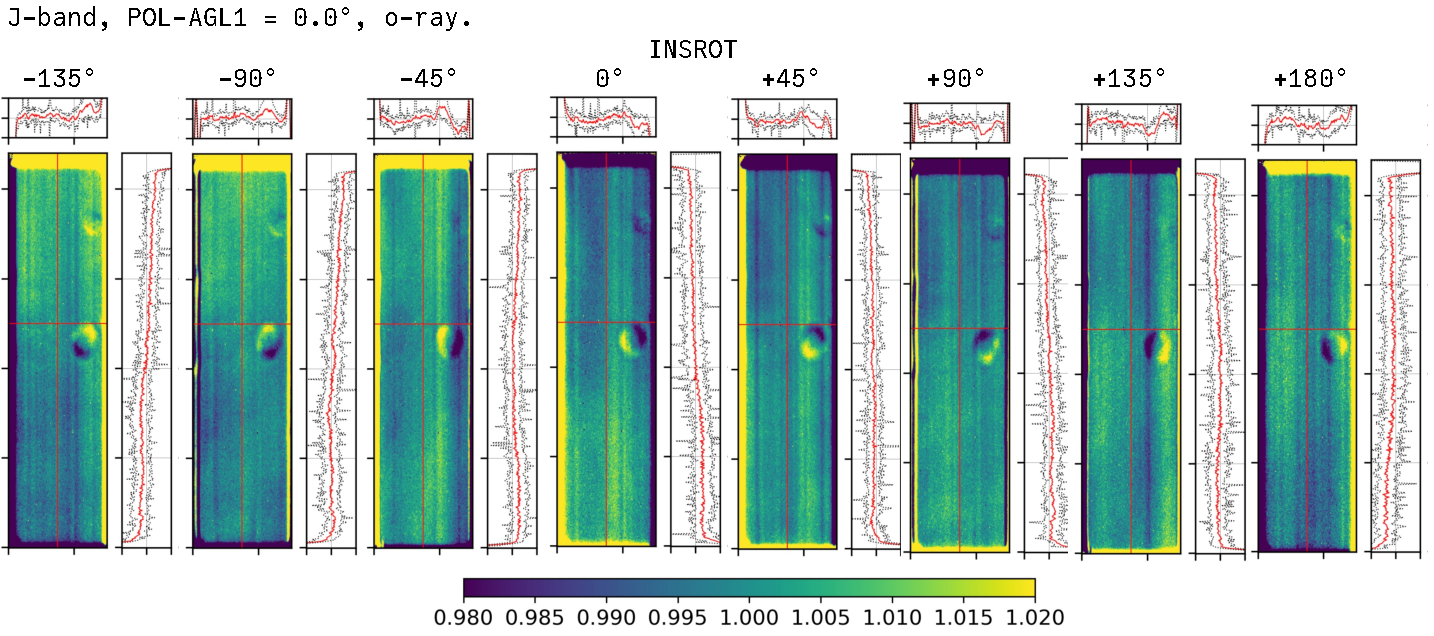
\includegraphics[width=\linewidth]{figs/flatinsrot.pdf}
  \end{center}
  \caption[The $ r_1 $ ratio map for J-band with HWP rotator angle $ 0^\circ $ and o-ray region only.]{Explanation, blah blah blah blah blah blah blah blah blah blah blah blah blah blah blah blah. Figure from \cite{2022_SAG_NICpolpy}.}
  \label{fig:flatinsrot}
\end{sidewaysfigure}



\begin{sidewaystable}[!ph]
  \centering
  \caption[Symbols frequently used in this paper.]{Explanation blah blah blah blah blah blah blah blah blah blah blah blah blah blah blah blah Table is from \cite{2019JKAS...52...71B}.}
  \label{tab: notation}
  \setlength{\tabcolsep}{19pt}
  \begin{tabular}{llll}
    \hline\hline
    Category & Symbols & Description & Value and Unit \\  % Table Heading
    \hline
    Magnitudes
     & $ V_\odot $         & Visual magnitude of the Sun           & $ -26.762 \mathrm{(mag)} $       \\
     & $ V $, $ \Delta V $ & Visual magnitude and its uncertainty  & $ \mathrm{(mag)} $ \\
     & $ \HVa $            & Reduced magnitude                     & $ \mathrm{(mag)} $ \\
     & $ \HV $             & Absolute magnitude ($ \coloneqq \HV(0) $) & $ \mathrm{(mag)} $ \\
     & $ G $               & Slope parameter                       & ~~ --- \\
    \hline
    Ephemerides
     & $ \rhel $, $ \robs $           & Heliocentric/geocentric distance          & $ \mathrm{m} $ or $ \mathrm{au} $ \\
     & $ \alpha $                 & Phase angle                               & ($ \mathrm{\degr} $ or $ \mathrm{rad} $) \\
     & $ t $                      & Time on the target (light-time corrected) & $ \mathrm{s} $ or $ \mathrm{JD} $ \\
     & $ (\lambda,\, \beta) $     & Ecliptic coordinate (longitude, latitude) & ($ \mathrm{\degr} $ or $ \mathrm{rad} $) \\
%     & $ (\lambda_\h,\, \beta_\h)_\mathrm{h.e.} $
%                                  & Heliocentric $ (\lambda, \beta) $         & ($ \mathrm{\degr} $ or $ \mathrm{rad} $) \\
%     & $ (\lambda_\g,\, \beta_\g)_\mathrm{g.e.} $
%                                  & Geocentric $ (\lambda, \beta) $           & ($ \mathrm{\degr} $ or $ \mathrm{rad} $) \\
%    \hline
%    Rotation
%     & $ \spin_1 $, $ \spin_2 $
%                                & Rotational/precessional vector              & ($ \mathrm{\degr} $, $ \mathrm{\degr} $)  \\
%     & $ P_1 $, $ P_2 $           & Rotational/precessional period            & $ \mathrm{s} $ or $ \mathrm{day} $ \\
%     & $ \omega_1 $, $ \omega_2 $ & Rotational/precessional angular speed     & $ \mathrm{s^{-1}} $ ($ \mathrm{rad/s} $) \\
%     & $ \varphi_1 $, $ \varphi_2 $ & Rotational/precessional phase offset    & ($ \mathrm{rad} $) \\
    \hline
    Physical
     & $ S_\mathrm{proj} $      & Total projected area viewed at $ \alpha = 0 $ & $ \mathrm{m^2} $ \\
    parameters
     & $ D $           & Effective diameter                                   & $ \mathrm{m} $ or $ \km $\\
     & $ \pV $         & Geometric albedo in visual (V) band                  & ~~ --- \\
     & $ A_5 $         & Albedo at the phase angle of $ \alpha = 5 \degr $    & ~~ --- \\
     & $ I $           & The irradiance of the object of interest             & $ \mathrm{W/m^2} $ \\
     & $ F $           & $ I $ of a Lambertian reflector at normal incidence  & $ \mathrm{W/m^2} $ \\
     & $ I/F $         & The radiance factor                                  & ~~ --- \\
    \hline
  \end{tabular}
\end{sidewaystable}



\chapter{Reference and Code}
\chapquote{He integrates empirically.}{Albert Einstein, {\footnotesize after saying ``God does not care about our mathematical difficulties.''}}
The reference in a PhD thesis can easily go beyond 100 items. The management will be tricky if you do not plan beforehand.

\section{Reference}
\subsection{ADS}
For astronomers, NASA provides a handy tool called ADS\footnote{\url{https://ui.adsabs.harvard.edu/}}, and its functionality, called ``Library'', is fantastic (though still in need of improvement). To use it efficiently, I have written a simple script called ``\texttt{ads2bibtex}''\footnote{\url{https://github.com/ysBach/ads2bibtex}}.


\subsection{Reference Style}\label{ss:ref style}
The reference style is nothing more than personal taste. Here I used the ``URL-ed A\&A style''\footnote{\url{https://github.com/yangcht/AA-bibstyle-with-hyperlink}}'' specified in the ``\texttt{aa\_url.bst}'' file. The \textcolor{magenta}{magenta link} redirects to the URL (usually DOI), and \textcolor{blue}{blue link} redirects to the ADS URL.
\textcolor{red}{I tweaked it a bit so that the bibliography shows the title of the publication in double quotes}.

\textbf{IMPORTANT NOTE}: As of 2023-05-18, at least \texttt{@PHDTHESIS} must have \texttt{adsurl=\{\}} and \texttt{adsnote=\{\}} if they are not registered with ADS. If you don't have these fields, you will get the following error:

  \texttt{Extra \}, or forgotten $\backslash$endgroup.}


\subsection{\texttt{cite}}\label{ss:cite}
You may already be familiar with citation. For your information:
\begin{itemize}[itemsep=-5pt, topsep=0pt, partopsep=0pt]
\item \texttt{cite} makes \cite{2021A&A...654A.113B}. If two arguments, \cite{2021A&A...654A.113B,2022MNRAS.509.4128I}.
\item \texttt{citet} makes \citet{2021A&A...654A.113B}. If two arguments, \citet{2021A&A...654A.113B,2022MNRAS.509.4128I}.
\item \texttt{citep} makes \citep{2021A&A...654A.113B}. If two arguments, \citep{2021A&A...654A.113B,2022MNRAS.509.4128I}.
\item \texttt{citealt} makes \citealt{2021A&A...654A.113B}. If two arguments, \citealt{2021A&A...654A.113B,2022MNRAS.509.4128I}.
\end{itemize}
With optional arguments, ``\texttt{$\backslash$citep[See, for example,][Figure 1]\{2021A\&A...654A.113B\}}'' becomes: \citep[See, e.g.,][Figure 1]{2021A&A...654A.113B}.


\section{\texttt{Cref}}\label{ss:cref}
\texttt{Cleveref} package provides multiple options for simple referencing. Please refer to the original documentation\footnote{\url{https://ctan.org/pkg/cleveref?lang=en}}.

\section{Code}
In this thesis, you can use \texttt{lstlisting} environment:

\begin{lstlisting}
# import nicpolpy package
import nicpolpy as nic

# Do not print useless warnings
import warnings
from astropy.utils.exceptions import AstropyWarning
warnings.filterwarnings('ignore',
    append=True, category=AstropyWarning)

# Cell 0: Initialize the reducer
npr = nic.NICPolReduc(
    name="SP_20190417",
    inputs="_original_32bit/190417/raw/*.fits",
    mflats="cal-flat_20180507-lv1/*.fits",
    imasks="masks/*.fits",
    verbose=1
)
\end{lstlisting}

You may modify the preference settings at the preamble in the ``\texttt{manuscript.tex}'' file.


\part{Journal Publications}\label{part-publications}
\chapter[Thermal Modeling of Comet-Like Objects from AKARI Observation]{Thermal Modeling of Comet-Like Objects from AKARI Observation\footnote{A version of this chapter has been published as \textbf{Bach, Y. P., Ishiguro, M., \& Usui, F. (2017) \textit{The Astronomical Journal}, 154, 202} \citep{2017AJ....154..202B}.}}\label{c:akari}
\section{Summary}
Summary of this paper. In the natural sciences, it seems to be customary to include published papers in the dissertation. Especially if the paper has already been published, you can (i) add a footnote to the chapter title to indicate the original publication and (ii) put the abstract of the paper in this ``Summary'' or ``Abstract'' section. You can just paste the content into the next sections.

\section{Future Work}
You can put the content of the published paper here. If you want, you can add additional comments, explanations, figures, tables, etc. that were not included in the original publication.

\chapter[Near Infrared Polarimetry of Airless Bodies Hints the Existence of Fine Dusts: The Case of Dawn Mission Targets, (4) Vesta and (1) Ceres]{Near Infrared Polarimetry of Airless Bodies Hints the Existence of Fine Dusts: The Case of Dawn Mission Targets, (4) Vesta and (1) Ceres\footnote{This work is currently ongoing and has not yet undergone peer review. A version of this chapter will be submitted to an academic journal in the near future, \textbf{Bach, Y. P., Ishiguro, M. \& Takahashi, J., et al. (2023), in prep. (to be submitted in mid to late 2023)}}}\label{c:nirpol}
\section{Summary}
It is not uncommon to include unfinished work in the dissertation. Especially if it is close to publication level, you can include it as a chapter, but indicate when it will be submitted/published.


\section{Future Work}
The draft of the contents (because it is an unpublished result) begins here.

\part{Concluding Remarks}\label{part-conclusion}
\chapter{Summary and Future Works}\label{c:summary}
\section{Summary}
Summary of this dissertaiton.

\section{Future Work}
Some possible future works:




%%%%%%%%%%%%%%%%%%%%%%%%%%%%%%%%% Bibliography %%%%%%%%%%%%%%%%%%%%%%%%%%%%%%%%%%%
\clearpage
\addcontentsline{toc}{chapter}{Bibliography}
\bibliographystyle{aa_url}
\setstretch{1.0}  % ← of course you can change this as you wish, too.
\bibliography{references.bib}
%%%%%%%%%%%%%%%%%%%%%%%%%%%%%%%%%%%%%%%%%%%%%%%%%%%%%%%%%%%%%%%%%%

%\appendix
%\chapter{Trailed Photometry}
%\input{chaps/trailed}




%%%%%%%%%%%%%%%%%%%%%%%%%%%%%%%%% 2nd Lang Abstract %%%%%%%%%%%%%%%%%%%%%%%%%%%%%%%%%%%
\setstretch{1.3} % ← of course you can change this as you wish, too.
\chapter*{한국어 초록}\addcontentsline{toc}{chapter}{한국어 초록}%\setcounter{page}{3}
{\small
\quad 본문이 비한국어인 경우 반드시 한국어 초록 첨부. (해당연도의 도서관 규정 필독). 폰트사이즈 일관성을 위해 여기 예시의 한국어초록은 ``$\backslash$\texttt{small}'' 사용.

~\\
\hangindent=2em
\hangafter=2
\textbf{주\,요\,어}: 소행성, 열적 모델링, 표토, 복사압, 편광---광학, 편광---적외선

~\\
\noindent \textbf{학 \quad 번}: 2016-20329
}

%%%%%%%%%%%%%%%%%%%%%%%%%%%%%%%%%%%%%%%%%%%%%%%%%%%%%%%%%%%%%%%%%%

%\chapter*{Acknowledgement}\\
%\twocolumn
\strangechapter{Ack}{Acknowledgement}\addcontentsline{toc}{chapter}{Acknowledgement}
\small
\footnotesize
\setstretch{1.1}
\setlength{\parskip}{0.3em}
Acknowledgement goes here. Hangul in Acknowledgement may use ``\texttt{$\backslash$kr}'': Hong Gildong (\kr{홍길동}).

ChatGPT says ``Both acknowledgment and acknowledgement are correct spellings. The only difference is that acknowledgment is the preferred American English spelling, while acknowledgement is the preferred British English spelling. You can use either one based on your preference or the style guide you're following.''



\end{document}
